\documentclass{article}
\setlength{\parskip}{5pt} % esp. entre párrafos
\setlength{\parindent}{0pt} % esp. al inicio de un párrafo
\usepackage{amsmath} % mates
\usepackage{url} % que las URLs se vean lindos
\usepackage[top=25mm,left=20mm,right=20mm,bottom=25mm]{geometry} % márgenes

\usepackage[utf8]{inputenc}
\usepackage[margin=1in]{geometry}
\usepackage{amsmath,amsfonts,amssymb,mathtools}
\usepackage{graphicx,float}
\usepackage{algorithmic}
\usepackage{minted}
\usepackage{subcaption}
\usepackage{multicol}
\usepackage{listings}
\usepackage{xcolor}
\usepackage[sort&compress,numbers]{natbib} % referencias
\usepackage{minted}
\usepackage{hyperref} % ligas de URLs
\usepackage{graphicx} % poner figuras
\usepackage[spanish]{babel} % otros idiomas
\usepackage{listings}
\author{Raul L.} % author
\title{Pr\'{a}ctica 5: Sistema Multiagente} %título
\date{\today}
\begin{document} % inicia contenido

\maketitle % cabecera


\section{Introducci\'{o}n}\label{intro} % sección y etiqueta



Un sistema multiagente es un poco como un autómata celular: hay un conjunto de entidades con estados internos que pueden observar estados de los otros y reaccionar cambiando su propio estado. La diferencia es que un sistema multiagente es un concepto más general y permite que estos agentes se muevan y varíen su vecindad, entre otras cosas. En esta práctica vamos a implementar un sistema multiagente con una aplicación en epidemiología. Los agentes podrán estar en uno de tres estados: susceptibles, infectados o recuperados, esto se conoce como el modelo SIR  \citep{ejemplo2}.

\section{Objetivo}
Estudia el efecto de contención en el sentido de que agentes infectados reduzcan su velocidad de movimiento a la mitad durante su infección. Determina con pruebas estadísticas adecuadas si este cambio produce un efecto significativo en la magnitud de la epidemia (la altura del pico en la curva del porcentaje de infectados por iteración) y en la velocidad de ella la iteración en la cual se llega por la primera vez al valor pico \citep{ejemplo2}.

\section{C\'{o}digo}
Para este código se utilizó como base el código de la doctora donde se hicieron modificaciones variando la velocidad para comprobar si afectaría en el porcentaje de contagios en el pico como también se agregaron un numero de repeticiones para poder tener una estimación considerable y poder hacer una correcta prueba estadística.

 Código en Python 

\url{https://github.com/satuelisa/Simulation/blob/master/MultiAgent/movement.py}

{\bf Código creado en Python}

\url{https://github.com/Raullr28/Resultados/blob/main/P4/codigo_celdas.py}

\renewcommand{\listingscaption}{Código}

\begin{listing}[H]
\begin{minted}{python}
if a.estado == 'I':
                    if div != 0:
                        x = a.x + (a.dx/div)
                        y = a.y + (a.dy/div)
                    elif div == 0:
                        x = a.x + (a.dx*div)
                        y = a.y + (a.dy*div)
                else:
                    x = a.x + a.dx
                    y = a.y + a.dy

  \end{minted}
  \label{lst:fibo}
  \caption{Representa la automatización para variar la velocidad de los infectados.}
  
  
\end{listing}
\renewcommand{\listingscaption}{Código}
\begin{listing}[H]

\begin{minted}{python}
 
for div in 1,2,0:
    print("####### velocidad 1/",div,"#########")
    pico, tmp= [], []
    for rep in range(repeticiones):
        agentes =  pd.DataFrame()
        agentes['x'] = [uniform(0, l) for i in range(n)]
        agentes['y'] = [uniform(0, l) for i in range(n)]
        agentes['dx'] = [uniform(-v, v) for i in range(n)]
        agentes['dy'] = [uniform(-v, v) for i in range(n)]
        agentes['estado'] = ['S' if random() > pi else 'I' for i in range(n)]
        epidemia = []
        for tiempo in range(tmax):
            conteos = agentes.estado.value_counts()
            infectados = conteos.get('I', 0)
            epidemia.append(infectados)
            if infectados == 0:
                break
  \end{minted}
  \label{lst:fibo}
  \caption{Representación función cambio de velocidad.}
\end{listing}

% Computational Results
\section{Resultados}
En las 3 figuras principales se muestra el comportamiento del pico con respecto a la reducción de la velocidad para demostrar como puede influir la velocidad de propagación en el pico de la pandemia, como prueba estadística se realizaron comparaciones con 30 repeticiones para cada caso de velocidad en graficas de caja-bigote.

\begin{figure}[H]
\centering
\begin{subfigure}[Absoluto]{0.40\linewidth}
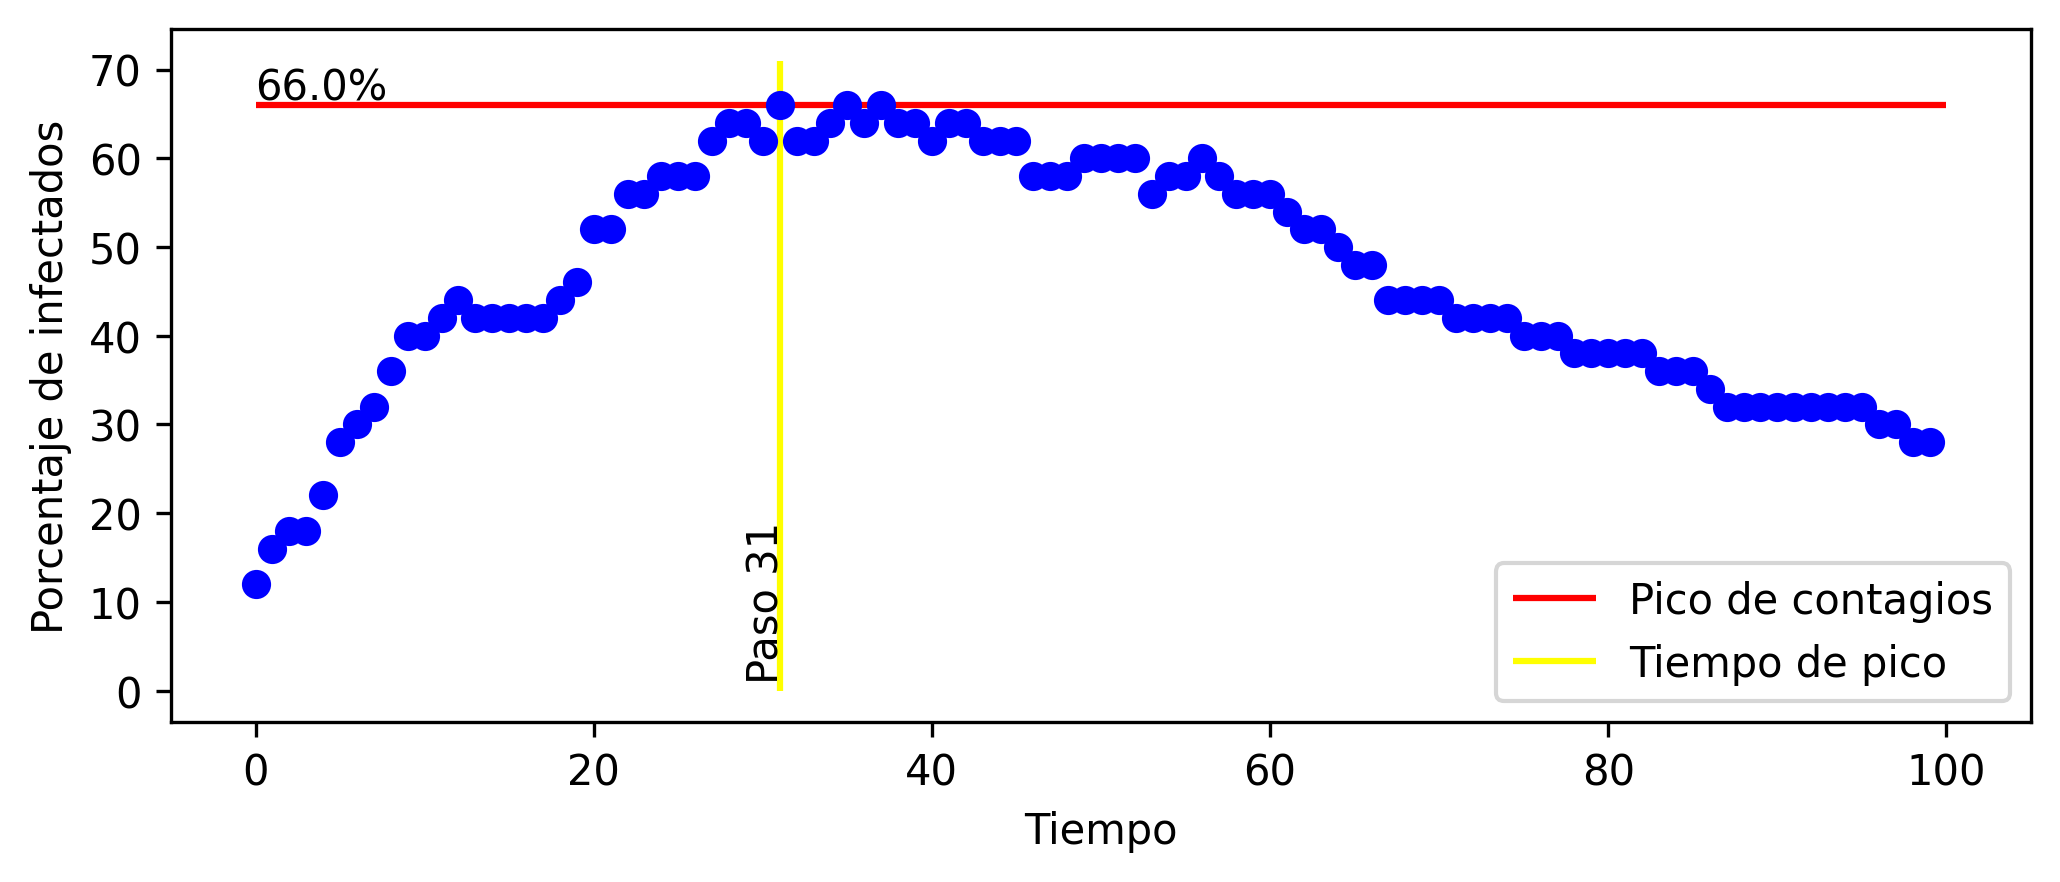
\includegraphics[width=\linewidth]{Imagenes/vel_normal.png}
\caption{Velocidad 1 }
\end{subfigure}
\begin{subfigure}[Cuadrado]{0.40\linewidth}
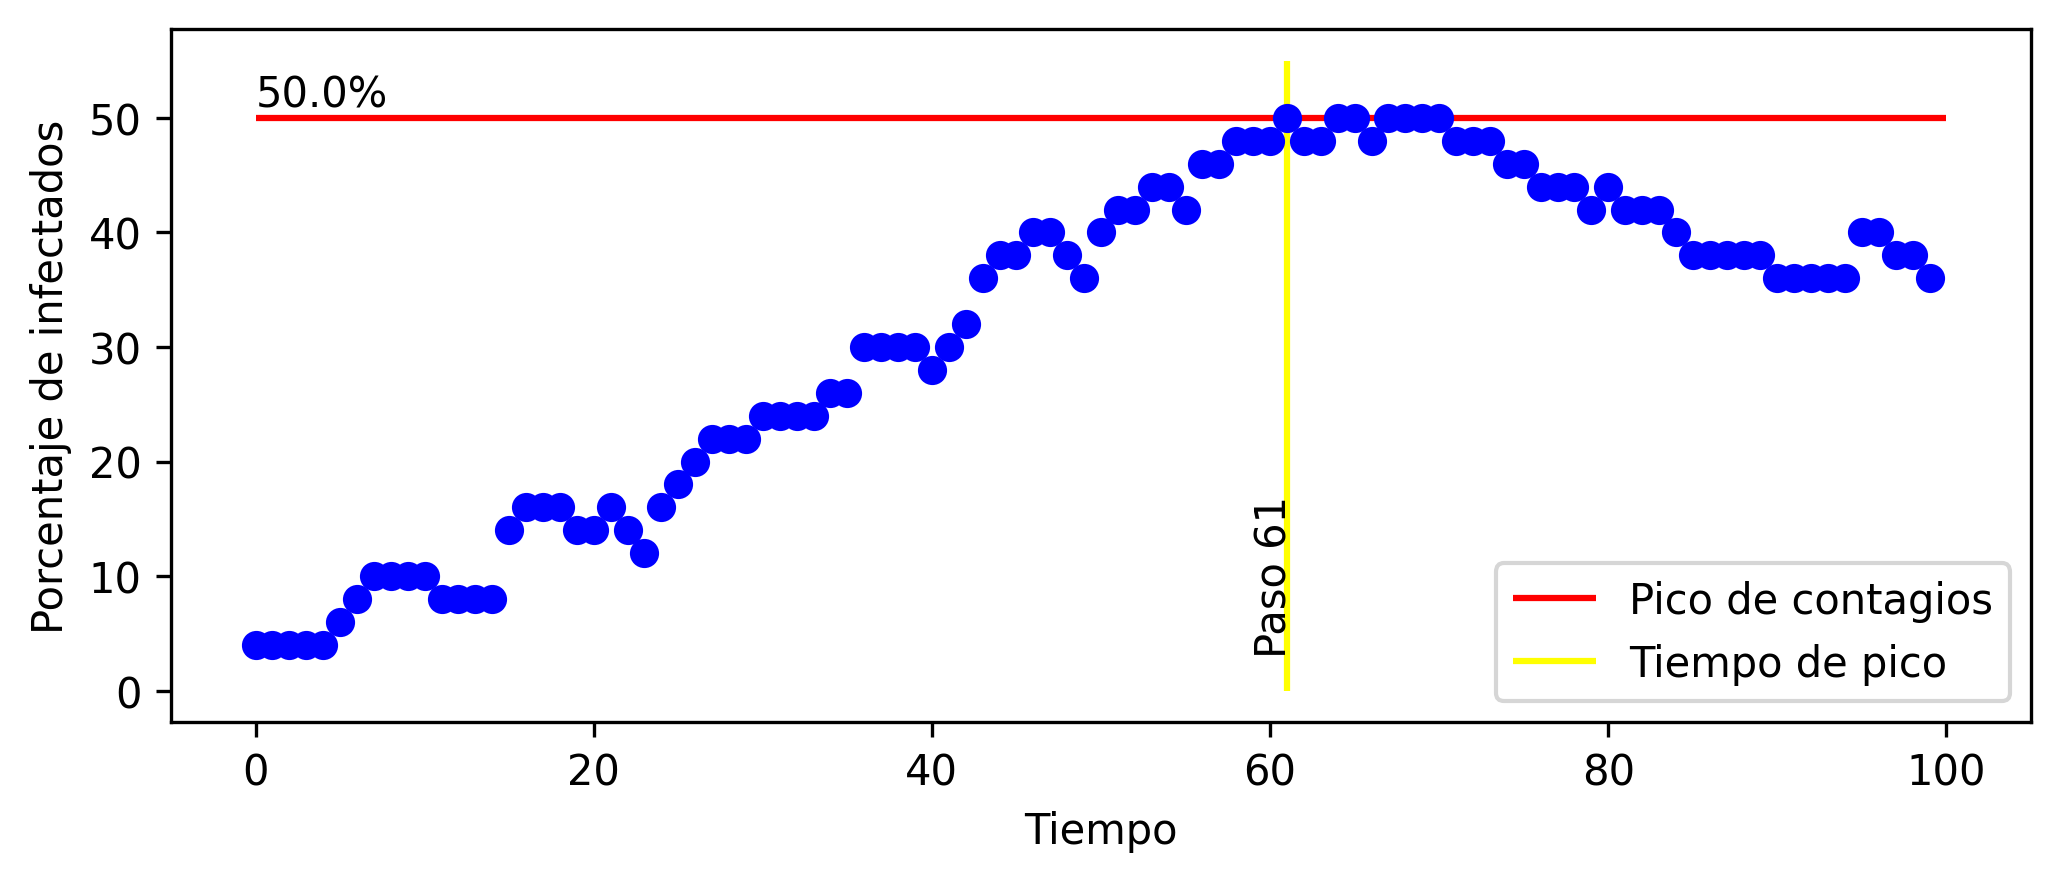
\includegraphics[width=\linewidth]{Imagenes/vel_1_2.png}
\caption{Velocidad 1/2}
\end{subfigure}
\caption{Gráfica de picos a diferentes velocidades.}
\label{fig:westminster}
\end{figure}

\begin{figure}[H]
\centering
\begin{subfigure}[b]{0.50\linewidth}
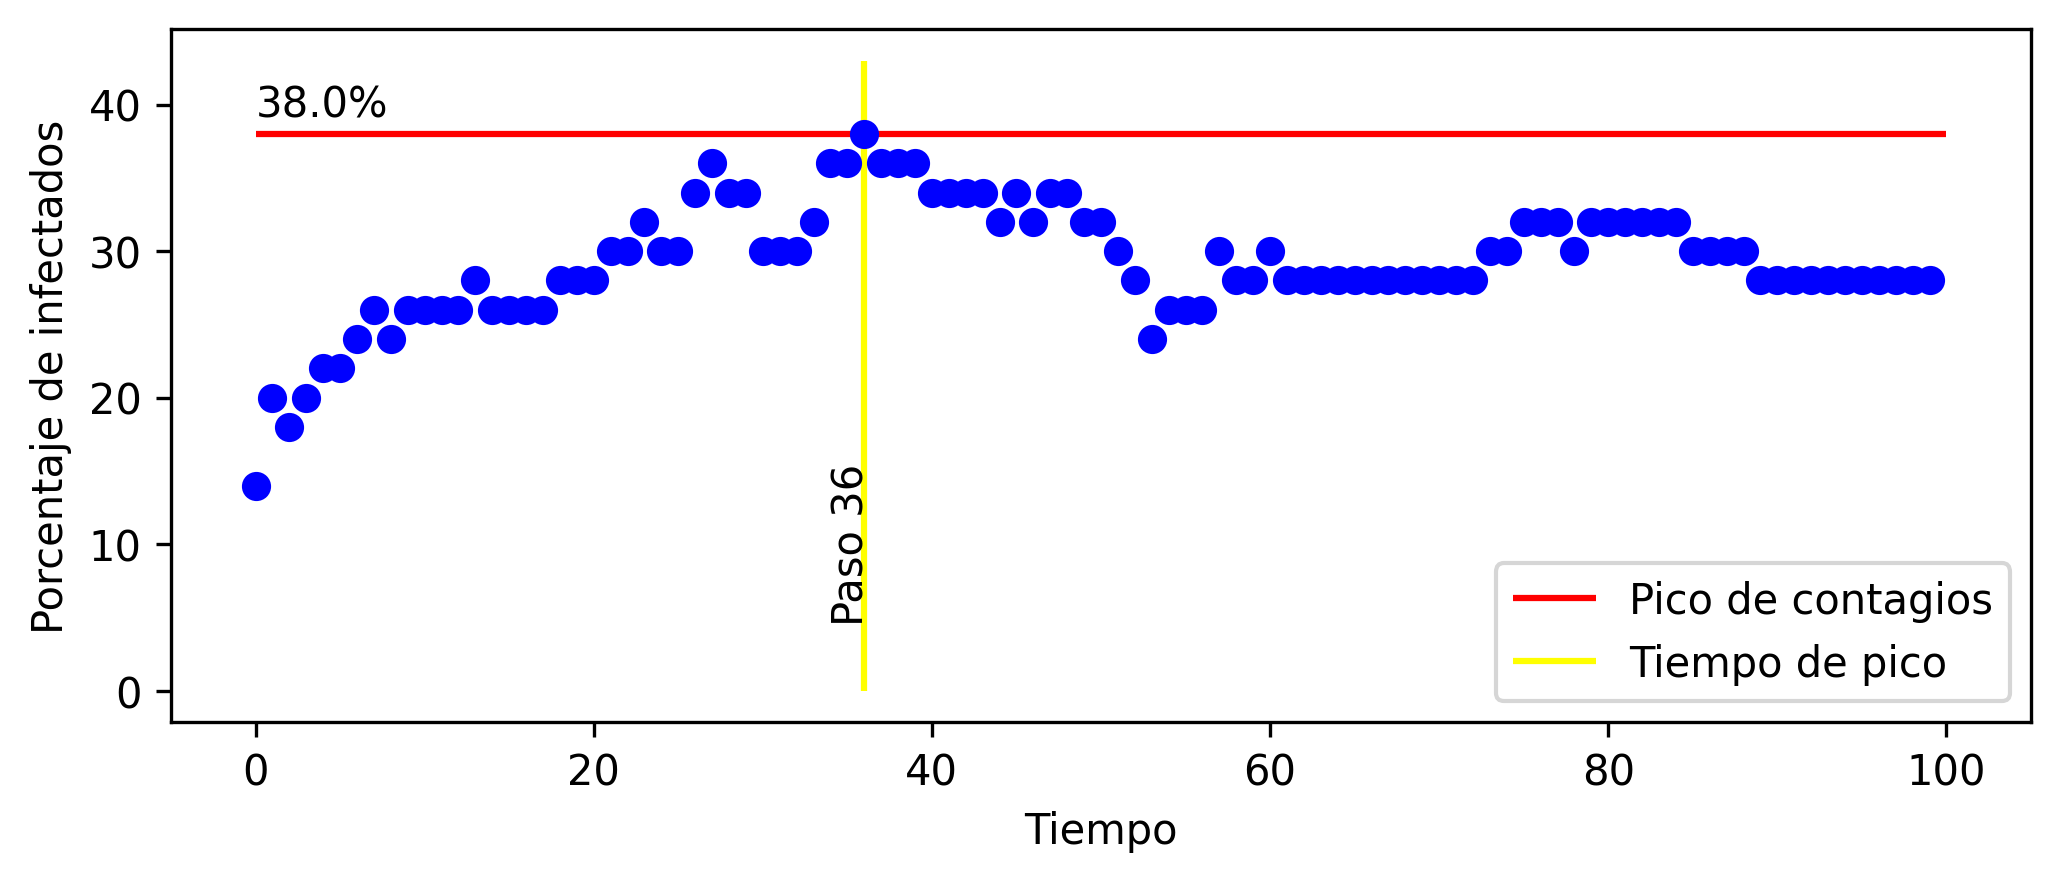
\includegraphics[width=\linewidth]{Imagenes/vel_nula.png}
\end{subfigure}
\caption{Velocidad nula 0.}
\label{fig:westminster}
\end{figure}

\begin{figure}[H]
\centering
\begin{subfigure}[Absoluto]{0.40\linewidth}
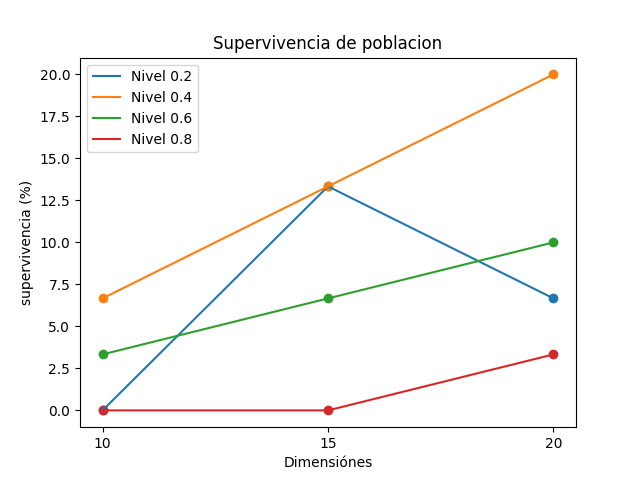
\includegraphics[width=\linewidth]{Imagenes/Figure_1.png}
\caption{Velocidad}
\end{subfigure}
\begin{subfigure}[Cuadrado]{0.40\linewidth}
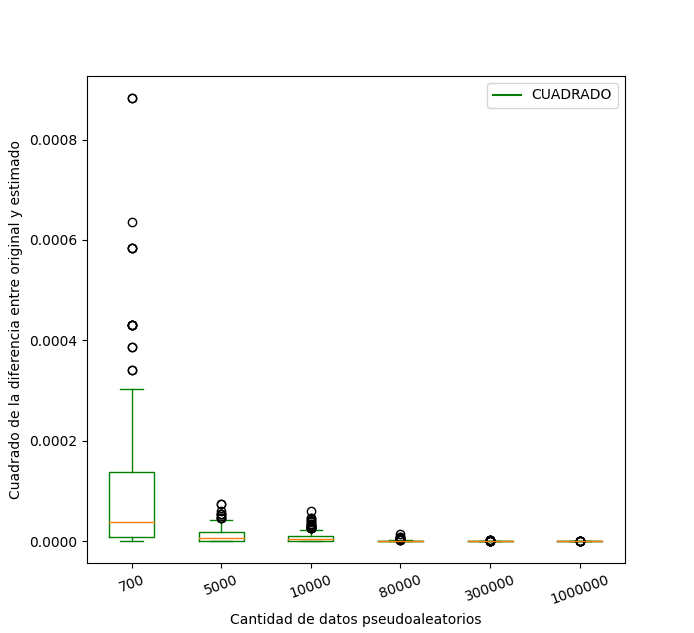
\includegraphics[width=\linewidth]{Imagenes/Figure_2.png}
\caption{Picos}
\end{subfigure}
\caption{Gráficas Estadisticas.}
\label{fig:westminster}
\end{figure}

\newpage
\section{Reto 1}
En el primer reto, vacuna con probabilidad 
 P{v} a los agentes al momento de crearlos de tal forma que están desde el inicio en el estado R y ya no podrán contagiarse ni propagar la infección. Estudia el efecto estadístico del valor de p{v} en (de cero a uno en pasos de 0.1) el porcentaje máximo de infectados durante la simulación y el momento (iteración) en el cual se alcanza ese máximo..

 
\section{Resultados}
 \begin{figure}[H]
\centering
\begin{subfigure}[b]{0.50\linewidth}
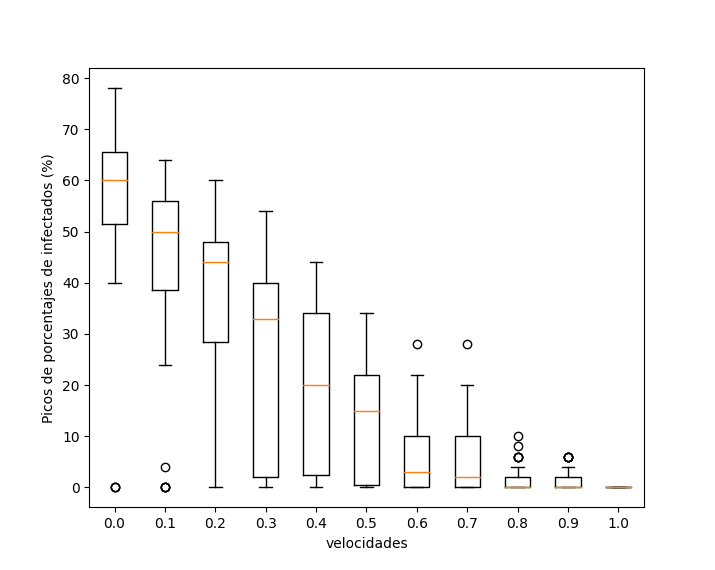
\includegraphics[width=\linewidth]{Imagenes/Figure_1_R.png}
\caption{porcentaje}
\end{subfigure}
\begin{subfigure}[b]{0.50\linewidth}
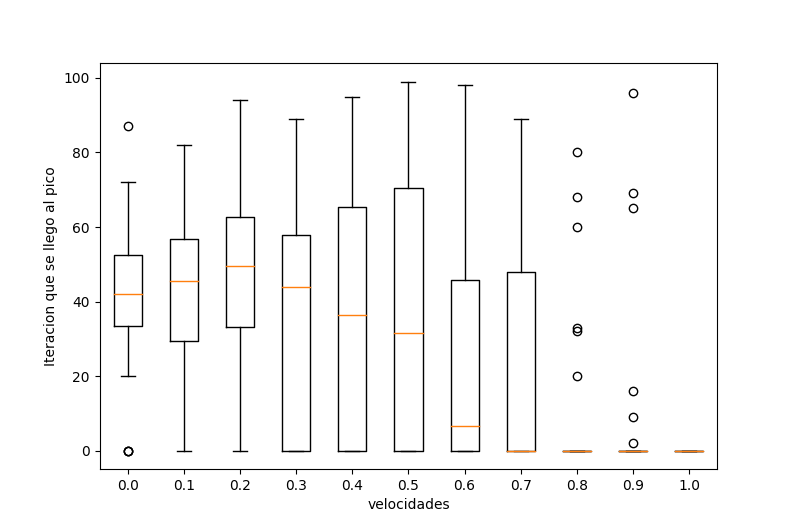
\includegraphics[width=\linewidth]{Imagenes/Figure_2_R.png}
\caption{Pico}
\end{subfigure}
\caption{Gráfica comparativa.}
\label{fig:westminster}
\end{figure}

\newpage
 \section{Conclusión}

Se demostró que disminuyendo la velocidad de los puntos como a su vez vacunando, hace que se reduzca la probabilidad de infectados y hace que arde en llegar más rápido el pico.

 \bibliography{bib.bib}
 \bibliographystyle{plainnat}

 \end{document}


